\documentclass[a4j,titlepage]{jarticle}
\usepackage[dvipdfmx]{graphicx}
\usepackage{ascmac}
\usepackage{url}

\title{呑兵衛土佐巡\\
画面遷移図\\
第2版}
\author{株式会社Spirytus}
\date{\today}

\begin{document}
\maketitle


\section{ユーザの画面遷移}

\begin {figure}[!htbp]
    \begin{center}
    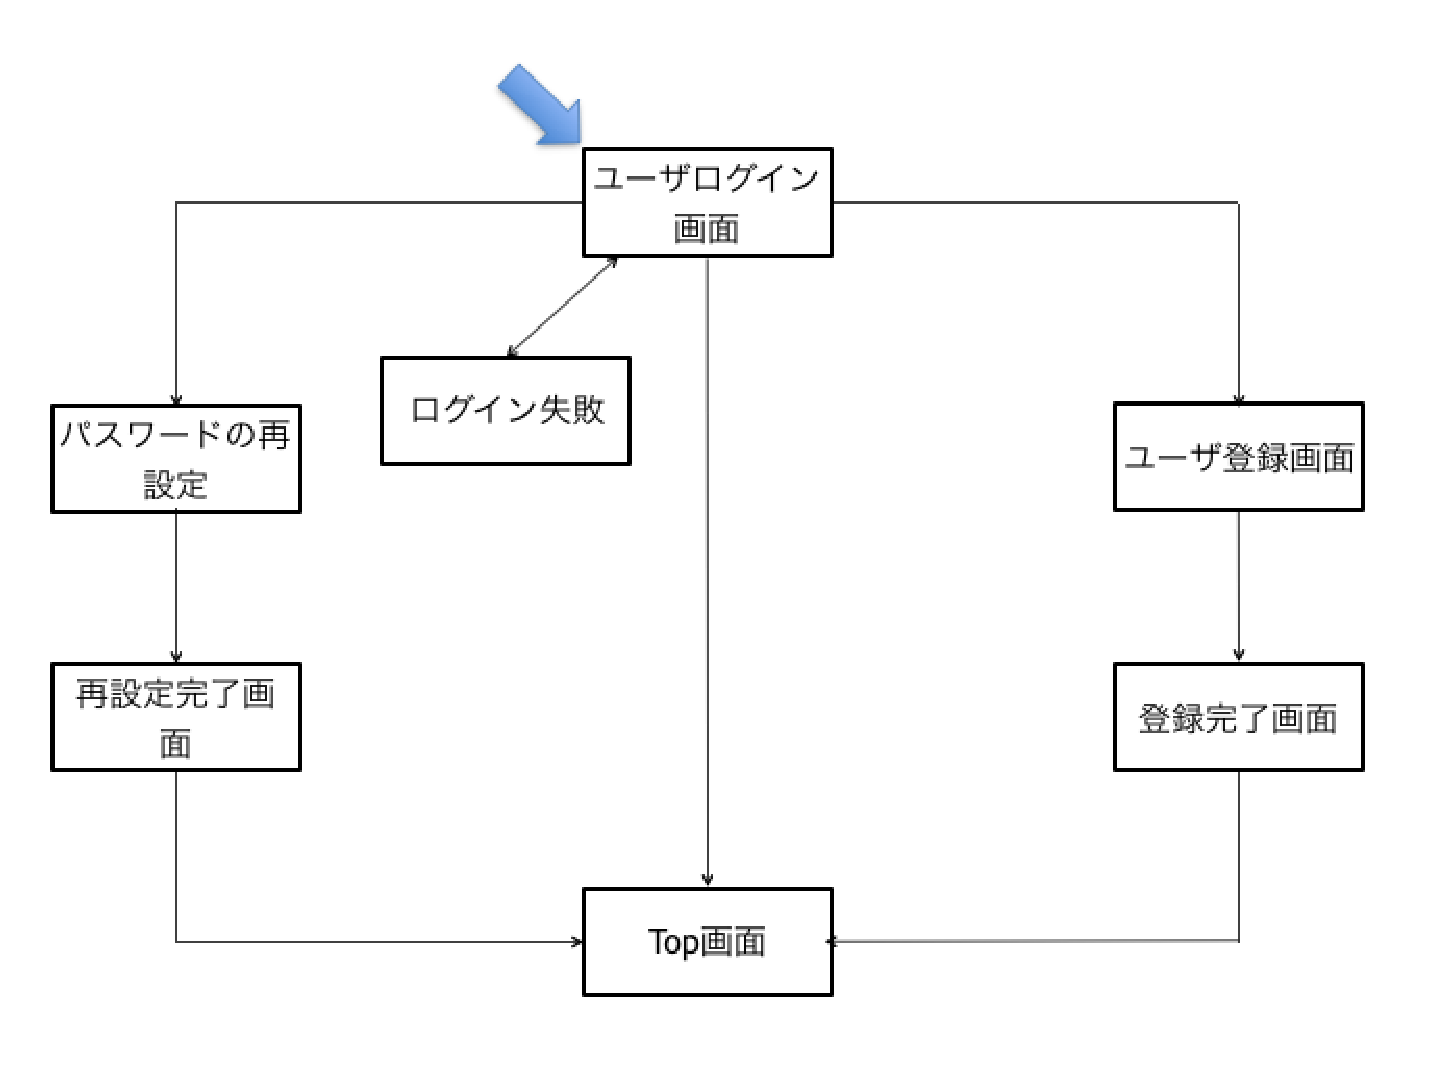
\includegraphics [height=7cm, width=8cm]{pass.eps}
    \caption {ユーザログイン画面からのユーザ登録とパスワード再設定の画面遷移図}
    \label {fig:pass}
    \end{center}
\end {figure}




\begin {figure}[!htbp]
    \begin{center}
    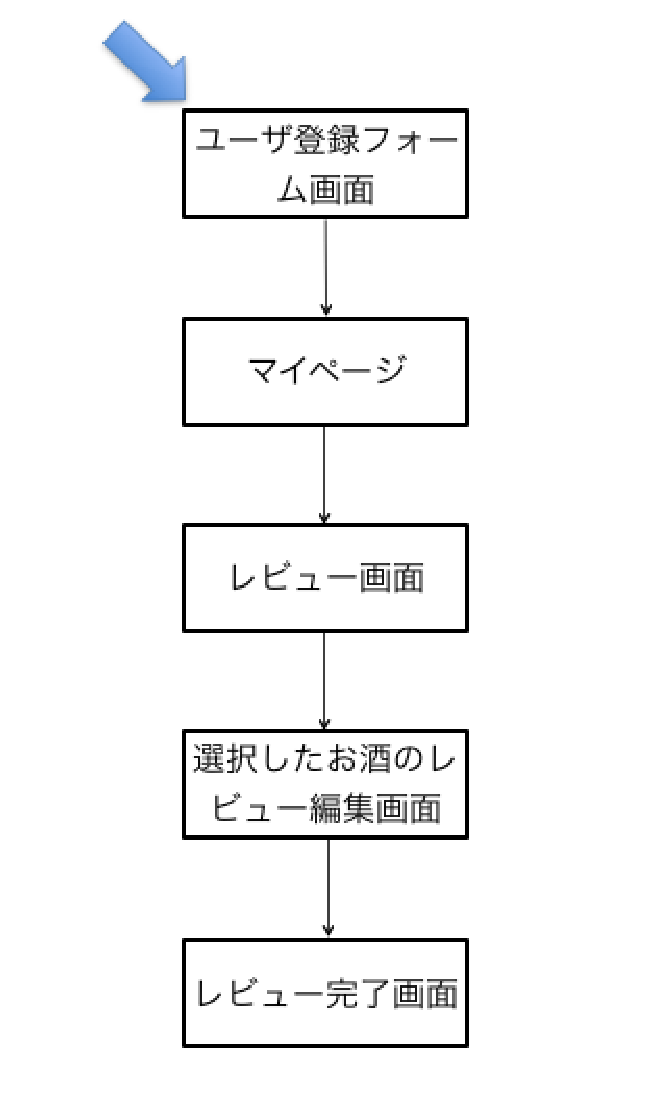
\includegraphics [height=8cm, width=6cm]{rebyu.eps}
    \caption {レビューの画面遷移図}
    \label {fig:rebyu}
    \end{center}
\end {figure}



\begin {figure}[!htbp]
    \begin{center}
    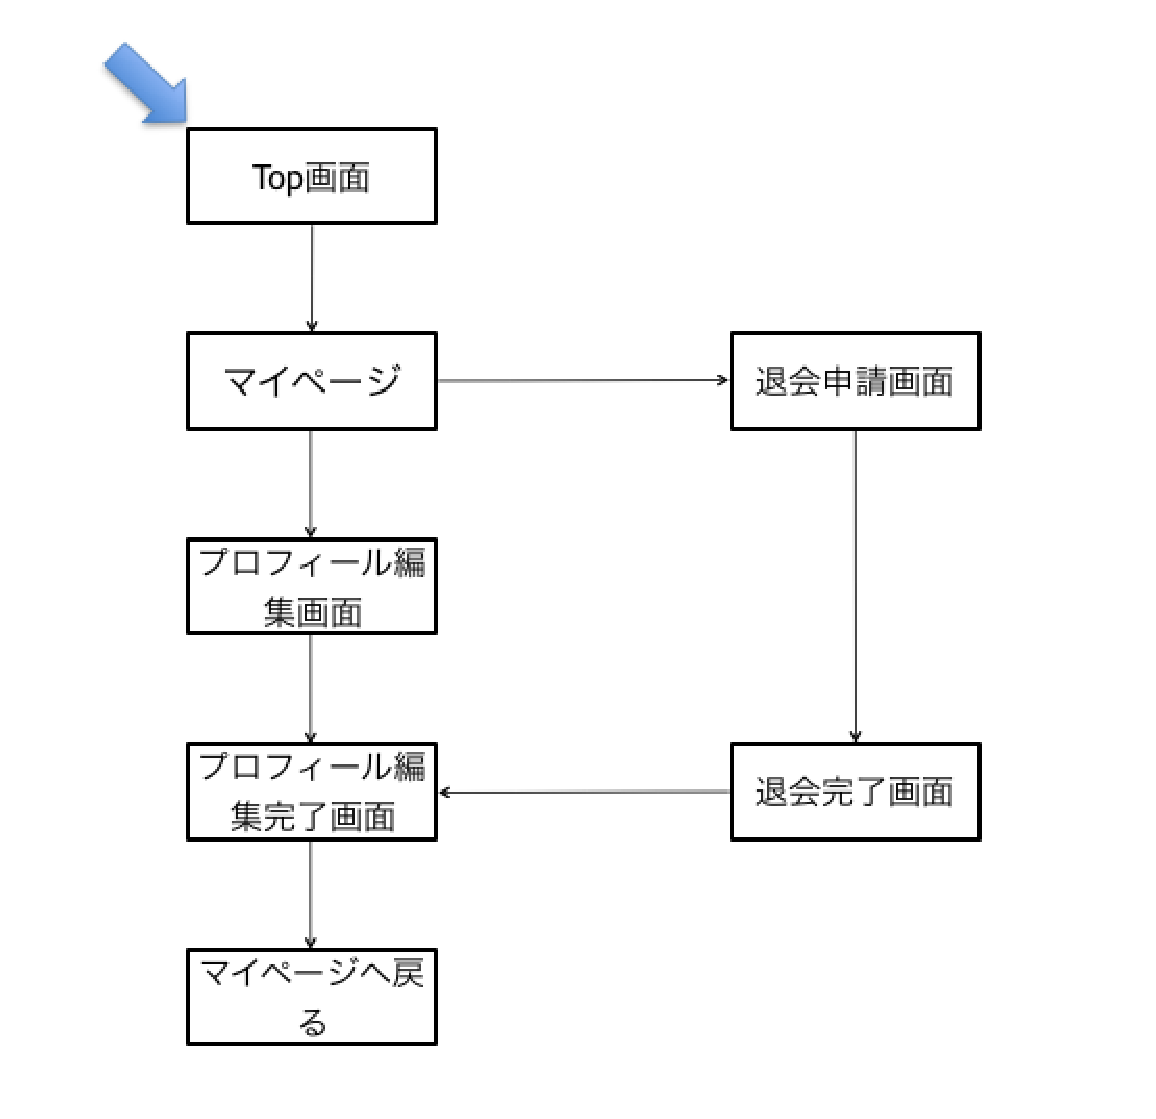
\includegraphics [height=7cm, width=7cm]{tai.eps}
    \caption {退会とプロフィール編集の画面遷移図}
    \label {fig:tai}
    \end{center}
\end {figure}

\clearpage


\section{店舗側の画面遷移}

\begin {figure}[!htbp]
    \begin{center}
    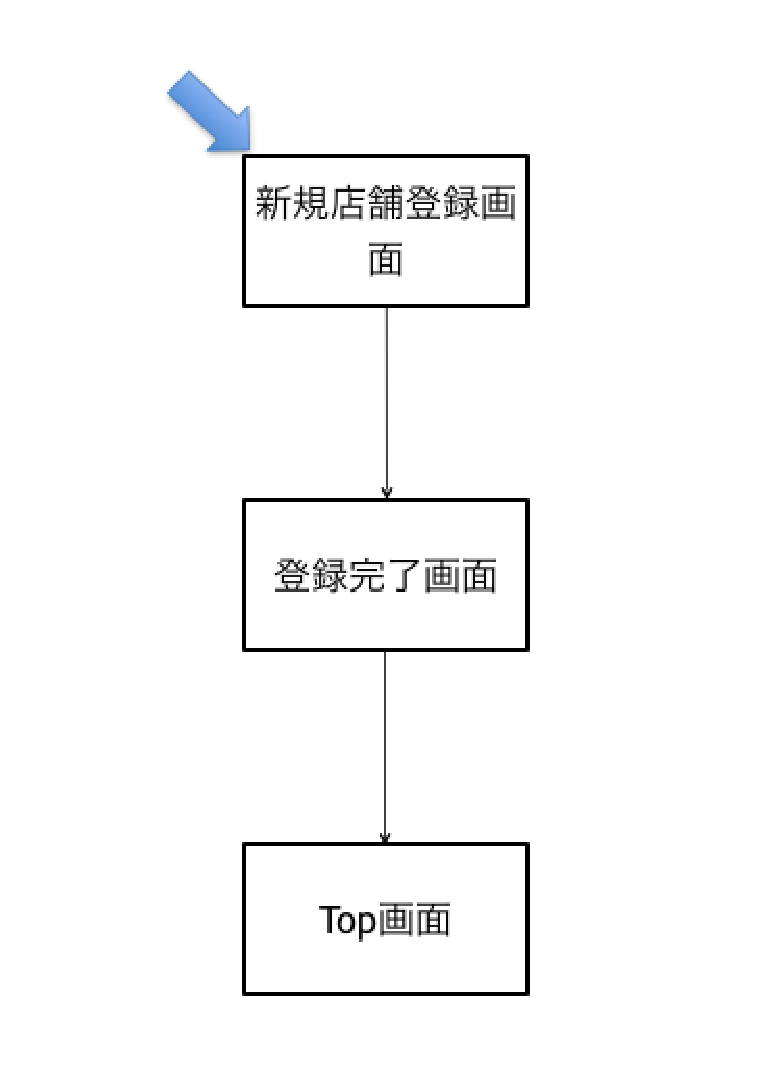
\includegraphics [height=7cm, width=6cm]{tenpo.eps}
    \caption {店舗登録の画面遷移図}
    \label {fig:tenpo}
    \end{center}
\end {figure}




\begin {figure}[!htbp]
    \begin{center}
    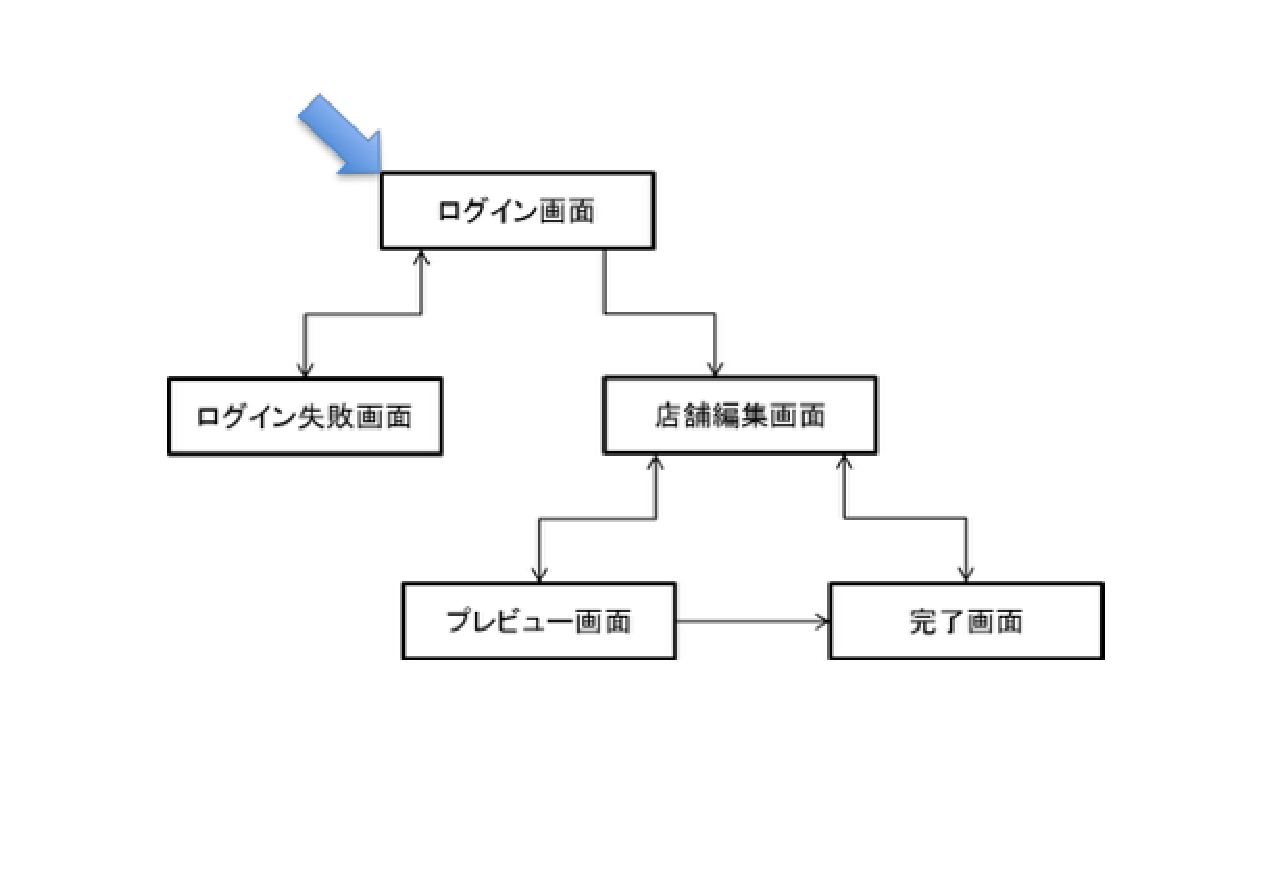
\includegraphics [height=8cm, width=8cm]{tere.eps}
    \caption {店舗編集の画面遷移図}
    \label {fig:tere}
    \end{center}
\end {figure}


\clearpage


\section{情報検索する画面遷移}

\begin {figure}[!htbp]
    \begin{center}
    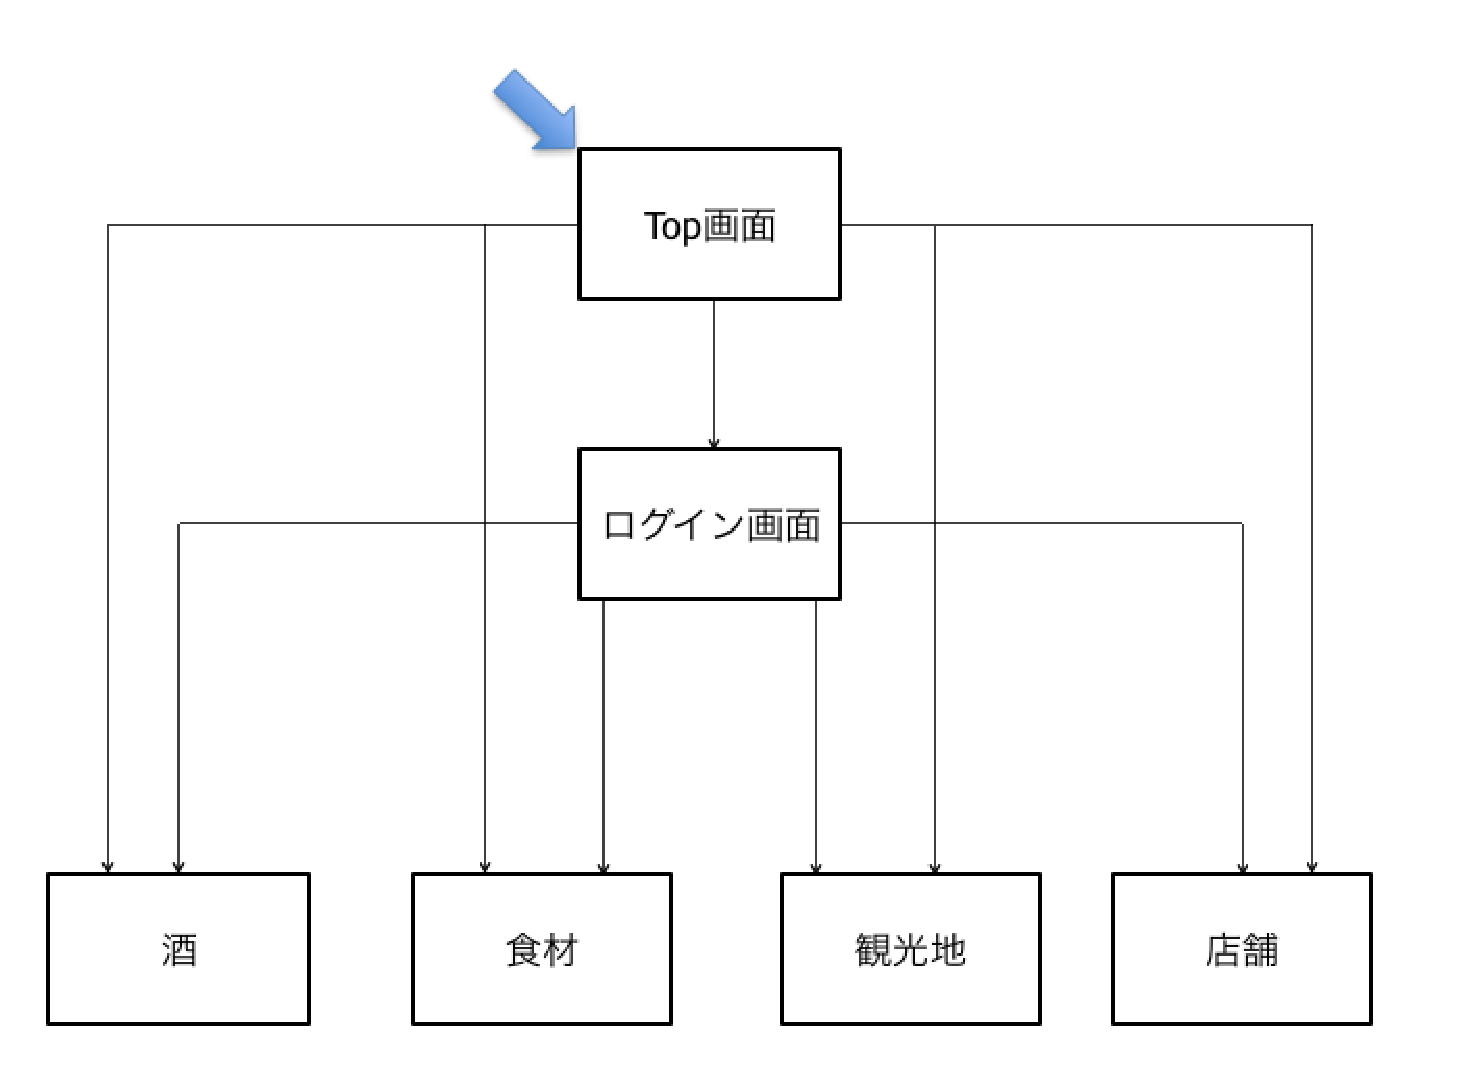
\includegraphics [height=7cm, width=8cm]{top.eps}
    \caption {Top画面、ログイン画面からの酒、食材、観光地、店舗の画面遷移図}
    \label {fig:top}
    \end{center}
\end {figure}



\begin {figure}[!htbp]
    \begin{center}
    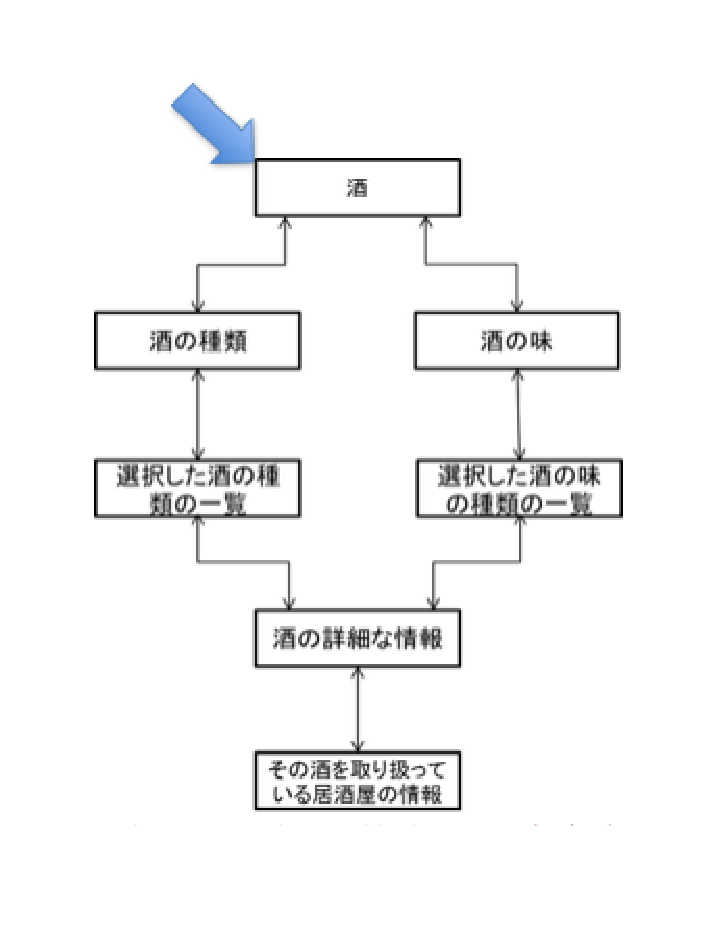
\includegraphics [height=8cm, width=7cm]{sake.eps}
    \caption {酒から居酒屋を検索する画面遷移図}
    \label {fig:sake}
    \end{center}
\end {figure}




\begin {figure}[!htbp]
    \begin{center}
    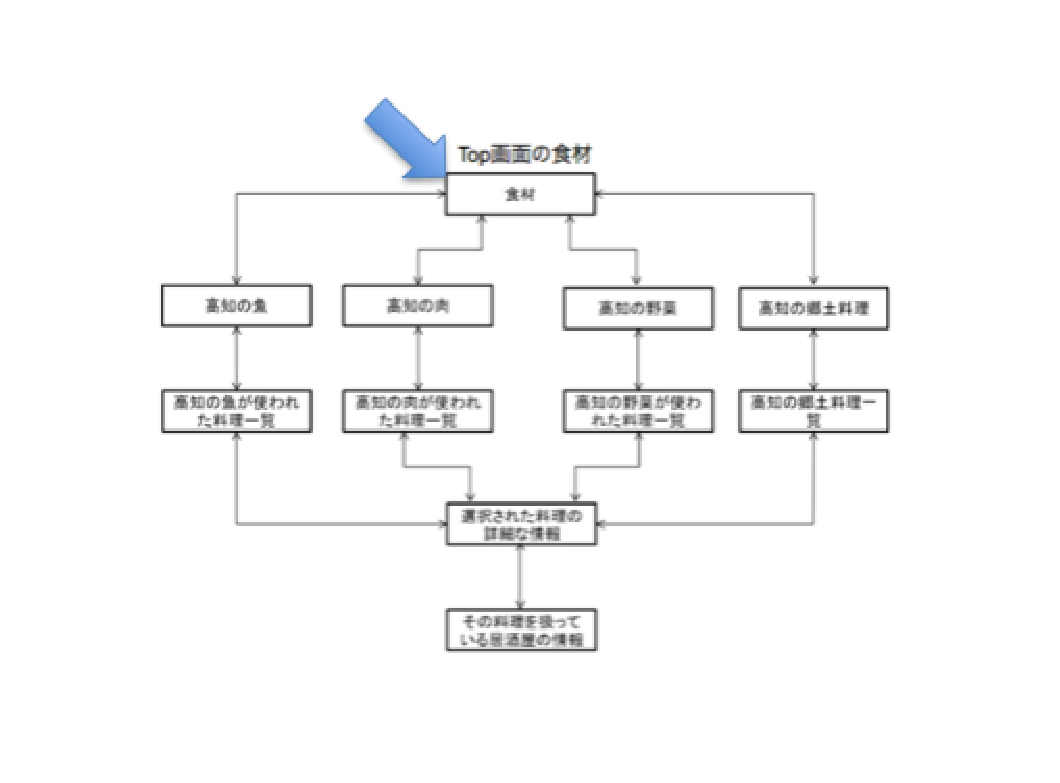
\includegraphics [height=9cm, width=9cm]{shokuzai.eps}
    \caption {高知の食材から居酒屋を検索する画面遷移図}
    \label {fig:shokuzai}
    \end{center}
\end {figure}




\begin {figure}[!htbp]
    \begin{center}
    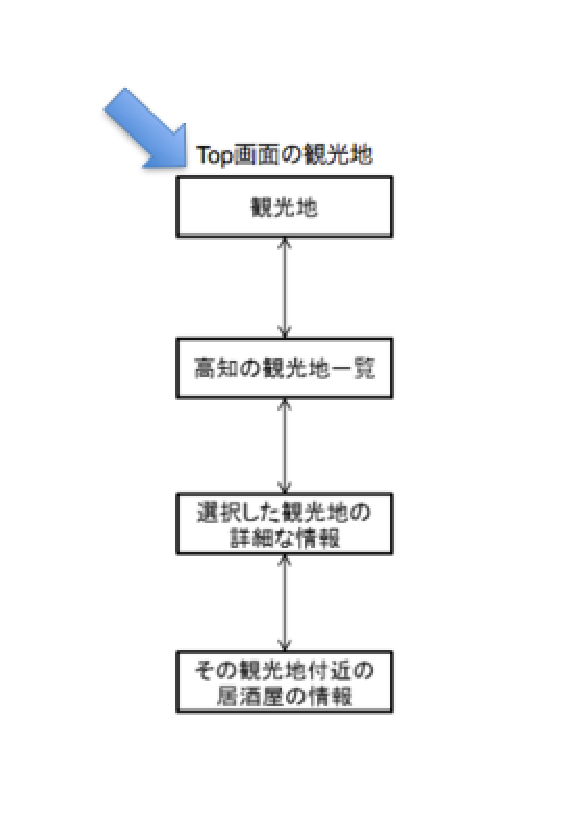
\includegraphics [height=8cm, width=6cm]{kankou.eps}
    \caption {高知の観光地から居酒屋を検索する画面遷移図}
    \label {fig:kankou}
    \end{center}
\end {figure}




\end{document}
